\documentclass[letterpaper,9pt,journal,final]{IEEEtran}

\usepackage{lmodern}
\usepackage{amssymb,amsmath}
\usepackage{ifxetex,ifluatex}
\usepackage{fixltx2e} % provides \textsubscript
\ifnum 0\ifxetex 1\fi\ifluatex 1\fi=0 % if pdftex
  \usepackage[T1]{fontenc}
  \usepackage[utf8]{inputenc}
\else % if luatex or xelatex
  \ifxetex
    \usepackage{mathspec}
  \else
    \usepackage{fontspec}
  \fi
  \defaultfontfeatures{Ligatures=TeX,Scale=MatchLowercase}
\fi
% use upquote if available, for straight quotes in verbatim environments
\IfFileExists{upquote.sty}{\usepackage{upquote}}{}
% use microtype if available
\IfFileExists{microtype.sty}{%
\usepackage{microtype}
\UseMicrotypeSet[protrusion]{basicmath} % disable protrusion for tt fonts
}{}
\usepackage[unicode=true]{hyperref}
\hypersetup{
            pdftitle={Tarea 1 - Procesamiento Digital de imágenes},
            pdfborder={0 0 0},
            breaklinks=true}
\urlstyle{same}  % don't use monospace font for urls
\ifnum 0\ifxetex 1\fi\ifluatex 1\fi=0 % if pdftex
  \usepackage[shorthands=off,main=spanish]{babel}
\else
  \usepackage{polyglossia}
  \setmainlanguage[]{spanish}
\fi
\usepackage{graphicx,grffile}
\makeatletter
\def\maxwidth{\ifdim\Gin@nat@width>\linewidth\linewidth\else\Gin@nat@width\fi}
\def\maxheight{\ifdim\Gin@nat@height>\textheight\textheight\else\Gin@nat@height\fi}
\makeatother
% Scale images if necessary, so that they will not overflow the page
% margins by default, and it is still possible to overwrite the defaults
% using explicit options in \includegraphics[width, height, ...]{}
\setkeys{Gin}{width=\maxwidth,height=\maxheight,keepaspectratio}
\IfFileExists{parskip.sty}{%
\usepackage{parskip}
}{% else
\setlength{\parindent}{0pt}
\setlength{\parskip}{6pt plus 2pt minus 1pt}
}
\setlength{\emergencystretch}{3em}  % prevent overfull lines
\providecommand{\tightlist}{%
  \setlength{\itemsep}{0pt}\setlength{\parskip}{0pt}}
\setcounter{secnumdepth}{5}
% Redefines (sub)paragraphs to behave more like sections
\ifx\paragraph\undefined\else
\let\oldparagraph\paragraph
\renewcommand{\paragraph}[1]{\oldparagraph{#1}\mbox{}}
\fi
\ifx\subparagraph\undefined\else
\let\oldsubparagraph\subparagraph
\renewcommand{\subparagraph}[1]{\oldsubparagraph{#1}\mbox{}}
\fi

\usepackage{url}


% set default figure placement to htbp
\makeatletter
\def\fps@figure{htbp}
\makeatother

\usepackage{booktabs}
\usepackage{flushend}
\makeatletter
\@ifpackageloaded{subfig}{}{\usepackage{subfig}}
\@ifpackageloaded{caption}{}{\usepackage{caption}}
\captionsetup[subfloat]{margin=0.5em}
\AtBeginDocument{%
\renewcommand*\figurename{Figure}
\renewcommand*\tablename{Table}
}
\AtBeginDocument{%
\renewcommand*\listfigurename{List of Figures}
\renewcommand*\listtablename{List of Tables}
}
\@ifpackageloaded{float}{}{\usepackage{float}}
\floatstyle{ruled}
\@ifundefined{c@chapter}{\newfloat{codelisting}{h}{lop}}{\newfloat{codelisting}{h}{lop}[chapter]}
\floatname{codelisting}{Listing}
\newcommand*\listoflistings{\listof{codelisting}{List of Listings}}
\makeatother

\title{Tarea 1 - Procesamiento Digital de imágenes}

\author{
            \IEEEauthorblockN{Pablo Yáñez S.}
        \IEEEauthorblockA{%
            % \\
            % \\
             - pablo.yanez@uai.cl}
        }

\date{}

\begin{document}
\maketitle


\hypertarget{selecciuxf3n-de-imagen}{%
\section{Selección de imagen}\label{selecciuxf3n-de-imagen}}

Para el desarrollo se utiliza un retrato encontrado en el sitio
\href{pexels.com}{www.pexels.com}. La fotografía presentanda en
la Figura ~\ref{fig:retrato}. fue tomada por Andrea Piacquadio
(\href{https://www.instagram.com/andreapiacquadio_/}{@andreapiacquadio\_}).

\begin{figure}[h!]
\hypertarget{fig:retrato}{%
\centering
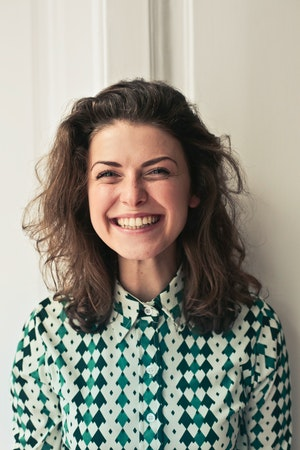
\includegraphics[width=0.2\textwidth]{portrait.jpg}
\caption{\href{https://www.pexels.com/photo/women-s-white-and-black-button-up-collared-shirt-774909/}{Retrato
a usar.}}\label{fig:retrato}
}
\end{figure}

Al estudiar los distintos canales de la imagen original se puede
apreciar que los canales azul y verde se parecen bastante, mientras que
el canal rojo se ve mucho más distinto que los otro dos. En especial en
este último se aprecian más pixeles con intensidades, especificamente en
la zona del rostro de la persona.

\begin{figure}[h!]
\hypertarget{fig:canales_retrato}{%
\centering
\includegraphics{outs/bgr.jpg}
\caption{Canales del retrato seleccionado.}\label{fig:canales_retrato}
}
\end{figure}

\hypertarget{equalizaciuxf3n-de-la-imagen}{%
\section{Ecualización de la imagen}\label{equalizaciuxf3n-de-la-imagen}}

La ecualización de los histogramas de la imagen corresponde al proceso
de modificar los valores de intensidad de la imagen, de modo que los
valores se encuentren en todo el rango. Esto permite que en la zonas de
bajo contraste este aumente.

\begin{figure}[h!]
\hypertarget{fig:canales_eq}{%
\centering
\includegraphics{outs/bgr_eq.jpg}
\caption{Ecualización de los canalaes de la
imagen.}\label{fig:canales_eq}
}
\end{figure}

En el resultado presentado en la Figura \ref{fig:canales_eq} se puede apreciar
que el canal que se mas afectado se vio por la ecualización es el canal
rojo.

\hypertarget{correciuxf3n-gamma}{%
\section{Corrección gamma}\label{correciuxf3n-gamma}}

Se aplica corrección gamma a cada uno del los canales de forma
independiente. Esto consiste en transformar cada uno de los valores de
cada unos de los pixeles de acuerdo a la siguiente función:

\[S = r^{\gamma}\]

Valores de \(\gamma < 1\) tiene el efecto de aumentar la intensidad de
los pixeles de la imagen, produciendo el efecto de ``aclarar'' la
imagen. Mientras que elegir valores \(\gamma > 1\) disminuyen la
intensidad de los pixeles, produciendo el efecto de ``oscurece'' la
imagen.

Dado que a priori se desconoce el valor de \(\gamma\) que se desea
aplicar a cada canal, se aplican valores entre \([0{.}5 - 1{.}9]\). A
modo de ejemplo en la Figura \ref{fig:gamma_red} se muestra la imagen
generada para el canal rojo.

\begin{figure}[h!]
\hypertarget{fig:gamma_red}{%
\centering
\includegraphics{outs/gamma_R_simple.jpg}
\caption{Ejemplo variación parámetro en corrección gamma para canal
rojo.}\label{fig:gamma_red}
}
\end{figure}

Luego de una inspección de los resultados para los distintos valores de
\(\gamma\) para cada uno de los canales se opta por elegir los valores
de \(\gamma_b=0{.}8\), \(\gamma_g=0{.}9\) y \(\gamma_r=1{.}2\) para cada
uno de los canales. El resultado obtenido para cada canal se presenta en
el la Figura \ref{fig:canales_gamma}.

\begin{figure}[h!]
\hypertarget{fig:canales_gamma}{%
\centering
\includegraphics{outs/gamma.jpg}
\caption{Correción gamma por canal.}\label{fig:canales_gamma}
}
\end{figure}

\hypertarget{filtro-de-la-mediana}{%
\section{Filtro de la mediana}\label{filtro-de-la-mediana}}

El filtro de la media es un filtro que se utiliza comúnmente para
reducir el ruido de una imagen. En este se reemplaza el valor de un
pixel en relación a sus vecinos. Los vecinos y el pixel se ordenan, y el
valor del pixel se reemplaza por el valor de la mediana del os datos. La
elección de la cantidad de vecinos se define en lo que se conoce como
máscara.

\begin{figure}[h!]
\hypertarget{fig:median_3}{%
\centering
\includegraphics{outs/median_3.jpg}
\caption{Filtro de la mediana por canal (3x3).}\label{fig:median_3}
}
\end{figure}

En la Figura \ref{fig:median_3} se presenta el resultado de aplicar un filtro
de la mediana con tamaño de máscara de 3x3. En comparación a la imagen
original, el resultado se ve como si estuviese suavizado, perdiendo
definición en los detalles. En especial se observa que se pierden
algunas de las imperfecciones presentes en el rostro.

\begin{figure}[h!]
\hypertarget{fig:median_5}{%
\centering
\includegraphics{outs/median_5.jpg}
\caption{Filtro de la mediana por canal (5x5).}\label{fig:median_5}
}
\end{figure}

Al agrandar la máscara del filtro se acentúa la difuminación de la
imagen. En la Figura \ref{fig:median_5} se puede nota se nota como se
empiezan a deformar las figuras geométricas de la blusa de la persona.

\hypertarget{imagen-final}{%
\section{Imagen final}\label{imagen-final}}

Utilizando las imágenes previamente generadas se genera una nueva imagen. En
la Figura ~\ref{fig:to_merge} se presentan las versiones a color de cada una
de las imágenes previamente generadas.


Realizando una suma ponderada de cada una de las imagenes se crea la imagen final. Se considera la siguiente ponderación para cada una de las imágenes:

\begin{itemize}
\tightlist
\item
  Imagen equalizada: 35\%
\item
  Imagen corrección gamma: 35\%
 \item
  Filtro de la mediana 3x3: 15\%
\item
  Filtro de la mediana 5x5: 15\%
\end{itemize}

\begin{figure}[h!]
\hypertarget{fig:to_merge}{%
\centering
\includegraphics{outs/color_merge.jpg}
\caption{imágenes a combinar.}\label{fig:to_merge}
}
\end{figure}


\begin{figure}[h!]
\hypertarget{fig:final}{%
\centering
\includegraphics{outs/before_after.jpg}
\caption{imagen original vs final.}\label{fig:final}
}
\end{figure}

En la Figura \ref{fig:final} se puede comparar el antes y después de la
imagen una vez que se han realizado todas las manipulaciones. Se puede
apreciar que cambia drasticamente la tonalidad de la imagen, pasando de
una tonalidad calida a una mas fría, cambios que se pueden atribuir a
las manipulaciones realizadas a través de la equalización y la correción
gamma. Las imperfecciones del rostro, especificamente en la zona de la
frente, se pierden gracias al efecto de los filtros de la mediana.

\hypertarget{manual-de-uso}{%
\section{Manual de uso}\label{manual-de-uso}}

En conjunto a este documento se entrega el código fuente asociado al
desarrollo de este trabajo.

Para recrear los resultados obtenidos en este documento basta con
ejecutar el script \texttt{Tarea\_1.py} agregando como opción la
pregunta asociada.

\begin{verbatim}
# Ejecuta pregunta 1
Tarea_1.py P1

# Ejecuta todo
Tarea_1.py ALL
\end{verbatim}


\end{document}
